The two sequential methods are implemented as separate functions that are called from within a while loop in the main file. The while loop runs as long as the checksum is larger than the threshold, $d$, AND while the number of iterations, $k$ is smaller than a user-specified $k_\mathrm{max}$:
\begin{lstlisting}
while(checksum > d && k < kmax)
\end{lstlisting}
The checksum is defined as the Frobenius norm of the difference between the updated matrix and the previous version of the matrix. The norm is
\begin{equation}
||u-u_O||_F = \equiv \sqrt{\sum_i\sum_j (u_{i,j}-u_{O, i,j})^2}.
\end{equation}
The functions are implemented in a straight-forward way with a double for loop. The input variables are the new matrix, $u$, the old matrix, $uo$, the source matrix, $f$, the size of the matrices, $N$, and the grid spacing squared $\Delta ^2$. The loops run from $1$ to $N-2$ such that the edge of the matrices are not updated.
\begin{lstlisting}[caption = Implementation of the sequential Jacobi iterative process]
void jacobi_seq(double ** u, double ** uo, double ** f, int N, double delta2){

	int i,j;
	for(i = 1; i < N-1; i++){
		for(j = 1; j < N-1; j++){
			u[i][j] = 0.25*(uo[i-1][j] + uo[i+1][j] + uo[i][j+1] + uo[i][j-1] + delta2*f[i][j]);
		}
	}
}
\end{lstlisting}

\begin{lstlisting}[caption = Implementation of the sequential Gauss-Seidel iterative process]
void gauss_seidel(double ** u, double ** f, int N, double delta2){

	int i,j;
	for(i = 1; i < N-1; i++){
		for(j = 1; j < N-1; j++){
			u[i][j] = 0.25*(u[i-1][j] + u[i+1][j] + u[i][j-1] + u[i][j+1] + delta2*f[i][j]);
		}
	}
}
\end{lstlisting}

\subsection{Comparing convergence}
The two functions are run with a fixed size of $N=100$, and $k_\mathrm{max}$ large enough that the clause that stops the while loop is always the convergence criterion. The threshold is varied from $10^{-1}$ to $10^{-11}$, and the resulting number of iterations until convergence fro the two functions is seen in figure \ref{fig:itd}. The $x$-axis is logarithmic, so the behavior is exponential, and the Gauss-Seidel is approximately twice as fast as the Jacobi method. The black dashed line is Jacobi line divided by two, and it follows the Gauss-Seidel line nicely.

\begin{figure}
\centering
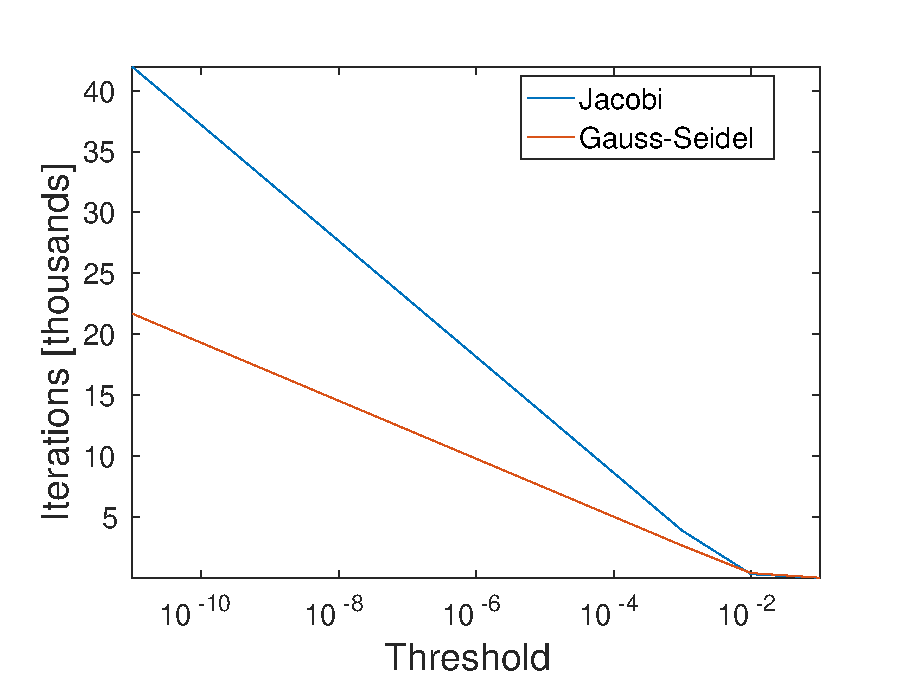
\includegraphics[width = 0.8\textwidth]{fig/itd_jac_gs.eps}
\caption{The convergence of the Jacobi method and the Gauss-Seidel method with changing threshold.}
\label{fig:itd}
\end{figure}